\subsection{Panorama Discovery}

Panorama discovery is defined as finding frames in a video that constitutes a panorama.  
Videos may contain frames that are not panoramic source images.  
We consider a video segment with the following properties to be a valid panorama source.  
A video segment is defined as a series of sequential frames.  There may be multiple video segments within a shot.

\vspace{5 mm}

\noindent\textbf{Property 1}: A video segment should cover a wide field-of-view based on the definition of panorama imagery.

\vspace{5 mm}

\noindent\textbf{Property 2}: A video segment should be �mosaicable�.  
Specifically, the underlying camera motion between frames should observe a certain camera motion model.  
We use a homography to model the motion between frames.  This property should be met after the shot detection algorithm.

\vspace{5 mm}

\noindent\textbf{Property 3}: The frames in a video segment should have high image quality.  
This conservative strategy is adopted so we can ignore methods to improve image visual quality, such as de-blurring and de-blocking.

\vspace{5 mm}

Ideally, we want to discover panoramas that have a very wide field-of-view and are of very high visual quality.  
Unfortunately, there is a tradeoff in practice.  More frames need to be included in order to have a wider field-of-view.  
However, including more source frames can often degrade the visual quality due to motion estimation error.  
We formulate discovering panoramas from a video shot as an optimization problem.  
The optimization problem aims to find a series of video segments that achieve an optimal balance between maximizing 
the visual quality of the resulting panoramas and maximizing the scenes they cover.  We implemented a variation
of the original optimization problem presented in the paper by Feng \cite{Feng}.  An overview of the orginal optimization problem is
described below followed by a detailed explaination of our modified optimization problem.  Lastly, our implementation
is discussed in greater detail.

\subsubsection{Original Optimization Problem}

The original optimization problem presented in the paper by Feng \cite{Feng} is shown in (\ref{eq:OrgOptEqu}).
Directly solving the constrained nonlinear programming problem is difficult.  
In fact the authors of the paper approximated the optimal solution.  Details of 
their approximation is discussed in paper.


% OPTIMIZATION PROBLEM
% FIRST LINE
\begin{equation} 
\hat{S}=arg min_{S}
\{ \sum_{S_{i}\epsilon S} E_{v}(S_{i}) + \sum_{S_{i},S_{j}\epsilon S} E_{a}(S_{i},S_{j}) \} \label{eq:OrgOptEqu}
\end{equation}
% SECOND LINE
\begin{equation*}
where \; S=\{ S_{i} \mid S_{i} \subseteq V \}, \;
\forall S_{i},S_{j} \epsilon S, \;
S_{i} \cap S_{j} = {\o}
\end{equation*}
% THIRD LINE
\begin{equation*}
s.t. \left\{ \begin{array}{l}
E_{v}(S_{i}) < \delta , \forall S_{i} \epsilon V \\
\varepsilon(S_{i}) > \beta A , \forall S_{i} \epsilon V
\end{array} \right.
\nonumber
\end{equation*}

\vspace{5 mm}

$S$ denotes a set that contains non-overlapping segments $S_{i}$ of the video clip $V$.
$E_{v}(S_{i})$ is the visual quality cost of stitching a panorama from $S_{i}$, and
$E_{a}(S_{i},S_{j})$ is the cost of splitting a panorama from $S_{i} \cup S_{j}$ into smaller
ones from $S_{i}$ and $S_{j}$ respectively.  $\varepsilon(S_{i})$ denotes the extent of the scene
in $S_{i}$, which is required to be bigger than $\beta$ times the original video frame
size $A$.  To gaurantee the visual quality of the panorama, the visual quality distortion
$E_{v}(S_{i})$ is required to be less than a threshold $\delta$.

\subsubsection{Modified Optimization Problem}

We relaxed the optimization problem as shown in equation (\ref{eq:OrgOptEqu}) to the two step problem shown in equations (\ref{eq:OurOptEqu1}) and (\ref{eq:OurOptEqu2}).
This difference provides our final algorithm with a major benefit.  The benefit is that $E_{a}(S_{i},S_{j})$, the cost of splitting a panorama, 
is no longer considered in Step 1, which reduces the computational difficulty.  Instead Step 2 aims to merge segments that greatly overlap.  
In our modified optimization problem we consider overlapping segments $S_{i}$ of the video clip $V$ as part of the set $S$.  The parameter $\alpha$
is used to tune the extent of overlap required for segments to be merged.  This is useful because to some extent identifying panoramas is
subjective to the user.  This will be discussed in greater detail in Section (\ref{sec:PanDiscExpSec}).


\vspace{5 mm}

\noindent\textbf{Step 1:}
% FIRST LINE
\begin{equation}
\hat{S}=arg min_{S} \{ \sum_{S_{i}\epsilon S} E_{v}(S_{i}) \} \label{eq:OurOptEqu1}
\end{equation}
% SECOND LINE
\begin{equation*}
where \; S=\{ S_{i} \mid S_{i} \subseteq V \} 
\end{equation*}
% FOURTH LINE
\begin{equation*}
s.t. \left\{ \begin{array}{l}
E_{v}(S_{i}) < \delta , \; \forall \; S_{i} \epsilon V \\
\varepsilon(S_{i}) > \beta A , \; \forall \; S_{i} \epsilon V
\end{array} \right.
\end{equation*}

\vspace{5 mm}

\noindent\textbf{Step 2:}
% FIRST LINE
\begin{equation}
P = 2^{S} \label{eq:OurOptEqu2}
\end{equation}
% SECOND LINE
\begin{equation*}
s.t. \{ \varepsilon(P_{i} \cap P_{j}) < min(\alpha \varepsilon(P_{i}),\alpha \varepsilon(P_{j})), \; \forall \; P_{i},P_{j} \epsilon V
\end{equation*}

\vspace{5 mm}

$S$ denotes a set that may contain overlapping segments $S_{i}$ of the video clip $V$.
$E_{v}(S_{i})$ is the visual quality cost of stitching a panorama from $S_{i}$.
$\varepsilon(S_{i})$ denotes the extent of the scene or total area in $S_{i}$, which is required to be bigger than $\beta$ times the original video frame
size $A$.  To gaurantee the visual quality of the panorama, the visual quality distortion
$E_{v}(S_{i})$ is required to be less than a threshold $\delta$.
$P$ is the power set of $S$ that meets the constraint of equation (\ref{eq:OurOptEqu2}).  The constraint is for any two subsets $P_{i},P_{j}$
of $P$, the area of their intersection must be less than $\alpha \varepsilon(P_{i})$ and $\alpha \varepsilon(P_{j})$.
P is the final set of panoramas, which may contain overlapping segments.

As mentioned, $E_{v}(S_{i})$ is the visual quality cost of stitching a panorama from $S_{i}$.  This is measured from two
aspects: the incorrectness of the motion model denoted as $E_{vm}(S_{i})$, and the source image visual quality distortion
denoted as $E_{vv}(S_{i})$.

\begin{equation}
E_{v}(S_{i}) = \alpha_{m} E_{vm}(S_{i}) + \alpha_{v} E_{vv}(S_{i}) \label{eq:Ev}
\end{equation}

\noindent where $\alpha_{m}$ and $\alpha_{v}$ are weights, with default values 1.0 and 1.0.

The motion model usually cannot be perfectly accurate when describing the correspondence between two frames.  Since we use
a homography for our motion model, homography error is used to measure the incorrectness of the motion model.  $E_{vm}(S_{i})$ is 
the sum of the homography errors between adjacent frames in $S_{i}$ as shown in equation (\ref{eq:Evm}).

\begin{equation}
E_{vm}(S_{i}) = \sum_{I_{k},I_{k+1} \epsilon S_{i}} H_{error}(I_{k},I_{k+1}) \label{eq:Evm}
\end{equation}

\noindent where $I_{k}$ is a frame and $H_{error}$ is the homography error between two adjacent frames.  Homography error 
calculation is discussed in Section (\ref{sec:HomoSec}).

Source frames often suffer from compression distortion.  We measure the input visual quality distortion using the blockiness and
blurriness discussed in Section (\ref{sec:BlurBlockSec}).  $E_{vv}(S_{i})$ is the sum of weighted blurriness extent and blockiness extent 
of each frame in $S_{i}$ as shown in equation (\ref{eq:Evv}).

\begin{equation}
E_{vv}(S_{i}) = \sum_{I_{k} \epsilon S_{i}} \gamma q_{bk}(I_{k}) + (1 - \gamma) q_{bk}(I_{k}) \label{eq:Evv}
\end{equation}

\noindent where $q_{bk}(I_{k})$ and $q_{br}(I_{k})$ measure the blockiness and blurriness of frame $I_{k}$, and 
$\gamma$ is a parameter with the default value 0.45.

\subsubsection{Implementation}

Our implementation is discussed in greater detail due to the complexity of the optimization problem.  The first step in our implementation is to
find the set $S$.  $S_{i}$ candidates are determined by selecting a reference frame as shown in Figure (\ref{fig:referenceFrame})
and then appending adjacent frames until the threshold $\delta$ is met.  All possible reference frames are considered to 
ensure a complete solution.  The set $S$ is determined from the set of $S_{i}$ candidates by verifying the scene extent is sufficient.
The second step is to merge video segements $S_{i}$ that greatly overlap.  The parameter $\alpha$ is used to tune the extent of overlap.
The set of segments $P$ are the discovered panoramas.

\begin{enumerate}
\item[I.] Determine the set $S$
\begin{enumerate}
\item[1.] Select a Reference Frame $I_{k}$ and place it in set $S_{i}$.
\item[2.] Determine the left most frame $I_{l}$ and right most frame $I_{r}$ in set $S_{i}$.
\item[3.] Find the minimum of $E_{v}(I_{l})$ and $E_{v}(I_{r})$.
\item[4.] Add $I_{l}$ or $I_{r}$ to the set $S_{i}$ depending on the results of the previous step.
\item[5.] Repeat steps 2 - 4 until the error threshold $\delta$ is met.
\item[6.] If $\varepsilon (S_{i}) > \beta A$ then add $S_{i}$ to $S$.  
\item[7.] Repeat steps 1 - 6 for all possible Reference Frames.
\end{enumerate}
\item[II.] Determine the set $P$
\begin{enumerate}
\item[1.] Find the power set of $S$ so that Equation (\ref{eq:OurOptEqu2}) is satisfied.
\end{enumerate}
\end{enumerate}

\begin{figure}[H] 
  \centering
  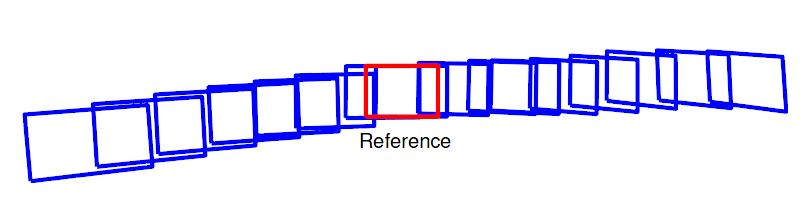
\includegraphics[scale=0.4]{referenceFrame.jpg}  
  \caption{All the frames in the video segment are aligned to the reference frame (in red).  
  The union of all these aligned quadrilaterals is the area covered by the video segment. \cite{Feng}} \label{fig:referenceFrame}
\end{figure}









